%\newcommand\tab[1][1cm]{\hspace*{#1}}
\chapter[Bunková biológia]{Bunková biológia}
\label{bunkova_biologia} % id kapitoly pre prikaz ref

%1
\subsection{Vnútorná organizácia buniek a ich pôvod v evolúcii DONE}
Status: DONE\\
Source: Prezentácia 1\\
\\
\subsection{História a kľúčové objavy bunkovej biológie}
Robert Hooke -- termín bunka, organizmy sú z buniek\\
Antonie van Leewenhoek -- mikroskop\\
\subsection{Bunková teória}
Schwann, Schleiden, Remak, Virchow\\
Pôvodné tri:\\
\tab Živé organizmy sú z jednej alebo viacerých buniek (dišputa -- vírusy)\\
\tab Bunky sú základné štruktúrne a funkčné jednotky živých organizmov\\
\tab Vznikajú len delením preexistujúcich buniek (Waaaait. Prvá bunka?)\\
Additional: \\
\tab Podobné chemické zloženie\\
\tab Chemický systém, kde prebieha premena energií a metabolické reakcie\\
\tab DNA je genetický materiál\\
\subsection{Porovnanie prokaryotických a eukaryotických buniek}
0.3 mikm -- 0.7 mm, 9 mikm -- 800 mikm\\
Prokaryotické\\
\tab Archaea, Bacteria\\
\tab Jadro (nucleoid) voľne v cytosole\\
\tab Bez membránových organel\\
\tab Cirkulárna DNA (cirkulárny chromozóm)\\
\tab Ribozómy\\
\tab Archaea má karboxyzómy, plynové vezikuly, etc.\\
Eukaryotické\\
\tab Eukarya\\
\tab Jadro má vlastnú membránu, nucleolus\\
\tab Membránové organely, napr. mitochondrie, golgiho aparát\\
\tab Viac vlákien DNA (viac chromozómov)\\
\tab Ribozómy\\
\subsection{Komplexná organizácia eukaryotickej bunky, význam intracelulárnej kompartmentalizácie a vnútrobunkový dialóg}
Bunková štruktúra -- Čokoľvek v bunke (ribozóm, deliace vretienko...)\\
Bunkový kompartment -- časť bunky oddelená membránou al. proteínom (cytosól, jadro)\\
Bunková organela -- funkčné časti bunky obklopené membránou (mitochondria, plastidy)\\
\\
jadro\\
mitochondrie, hydrogenozómy\\
plastidy (rastlinné bunky)\\
endoplazmatické retikulum\\
Golgiho aparát\\
lyzozómy, vakuoly\\
peroxizómy\\
cytosol\\
\subsection{Vznik buniek v evolúcii}
RNA(Genotyp + Fenotyp) $\rightarrow$ RNP(Genotyp + Fenotyp) $\rightarrow$ DNA(Genotyp ~ DNA + Fenotyp(Proteínový))\\
Darwin\\
\tab jeden spoločný predok\\
Woese\\
\tab viacero vetiev $\rightarrow$ tree of life, archaea, bacteria, eucarya\\
\tab RNA selfreplicating teória\\
Darwinovský prah (Darwinian Treshold) -- bod, pred ktorým speciácia nebola možná, kvôli horizontálnemu transferu génov\\
\subsection{Pôvod komplexnej (eukaryotickej) bunky}
Lynn Margulis\\
Endosymbiotická teória\\
Evolučná mozaika\\
Niektoré organely (mitochondrie, plastidy) vznikli vďaka endosymbióze. Resp. eukarya vznikli ako symbióza archaea a procarya. Jadrový genóm pochádza z archaea a bacteria...\\
Reduktívna fáza -- strata časti genómu, funkcií, transfer génov do jadra\\
Expanzívna fáza -- vznik nových génov, horizont. gén. transfer prokaryotických génov, konverzia endosymbionta na organelu exportujúcu ATP\\
Mitochondrie majú vlastný genóm\\
Vodíková hypotéza\\

%2
\section{Bunkové jadro: štruktúra a dynamika chromozómov}
Status: In progress\\
Source: Prezentácia 2\\

\subsection{Prokaryotické, eukaryotické a organelové chromozómy}
Prokaryotické, organelové\\
\tab jedna cirkulárna molekula DNA, kondenzáciu zabezpečuje viacero proteínov\\
\tab nucleoid\\
\tab ribozómy voľne v cytoplazme\\
Eukaryotické\\
\tab väčšinou viacero chromozómov -- 1 chromozóm = 1 DNA\\
\tab zabaľovanie -- históny, ďalšie proteíny\\
\tab nucleus\\
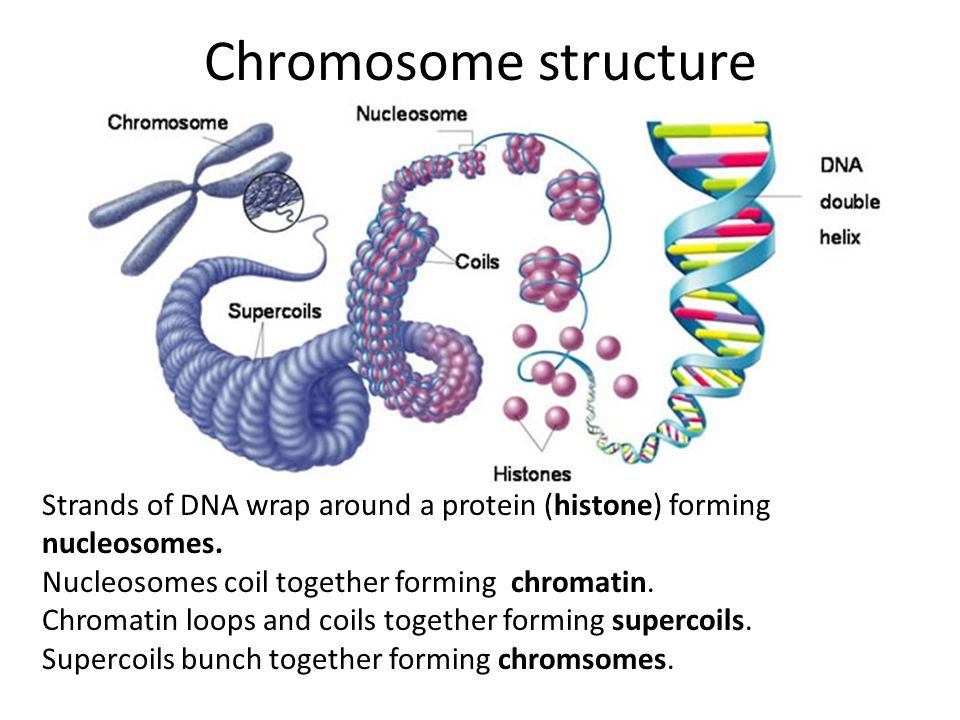
\includegraphics[width=0.2\textwidth]{images/bunkova_bio/chromosome_dna}\\

\subsection{DNA a proteínové komponenty chromozómov}
Históny -- alkaline structure proteins\\
DNA\\
\subsection{Distribúcia chromozómov pri delení buniek}
rovnomerne distribuované do dcérskych buniek\\
$G_1$ fáza -- bunka rastie\\
$S$ fáza -- chromozómy sa zdvoja \ra sesterské chromatídy\\
$G_2$ fáza -- zase rastie\\
Mitóza -- delenie\\
\tab centrozómy idú na opačné strany bunky a roztiahnu chromatídy od seba\\
\subsection{Objav úlohy DNA}

\subsection{Replikačné stratégie DNA}

\subsection{Experimenty Meselsona a Stahla}

\subsection{Semikonzervatívny mechanizmus syntézy DNA}

\subsection{Iniciácia, elongácia a terminácia replikácie (replikačné počiatky, replikačné bubliny}

\subsection{Okazakiho fragmenty, leading a lagging vlákno). Replizóm}

\subsection{Kľúčové enzýmy v replikácii: DNA polymerázy, primázy, ligázy, helikázy, topoizomerázy, ssb proteíny}

%3
\section{Mechanizmy opravy poškodenej DNA DONE}

Status: DONE\\
Source: Prezentácia 3\\

Typy: Na svetle / v tme, počas replikácie / po replikácii, error free / error prone\\
3' $\rightarrow$ 5' je nevýhodné, lebo pri napájaní sa nerozpadne väzba, ktorá by poskytla energiu na polymerizáciu (odštiepenie fosforov)\\

\subsection{Poškodenia chromozomálnej DNA}
Poškodenia: chemické modifikácie, straty báz, pyrimidínové diméry, krížové väzby v DNA, zlomy\\
Depurinácia -- Príde voda, odíde báza\\
Deaminácia -- Príde voda, odíde NH3, báza sa zmení na inú (cytozín $\rightarrow$ uracil)\\
lézia -- poškodenie $\rightarrow$ fixácia $\rightarrow$ mutácia\\
\subsection{Fyzikálne, chemické a biologické mutagény}

\subsection{Príčiny vzniku spontánnych mutácií}

\subsection{Reparačné mechanizmy (fotoreaktivácia, bázová a nukleotidová excízna reparácia, rekombinačná oprava, SOS odpoveď)}

Tymínové diméry -- oprava na svetle (UV) fotoreaktívnym enzýmom
Demetylácia / dealkylácia -- oprava enzýmom

Bázová excízna oprava (deamiated C)-- najprv odíde báza, potom cukor, potom DNA polymeráza doplní 1, DNA ligáza zalepí dokopy\\
Nukleotidová excízna oprava (napr. pyrimid. dimér) -- nukleáza rozštikne, DNA helikáza oddelí, DNA polymeráza doplní väčší úsek\\
Starý úsek je metylovaný napr. na konkrétnej sekvencii\\

opravy dvojvláknových zlomov rekombináciou\\
\tab Nehomologické -- zožerie nukleotidy na konci zlomu Non-homologous end joining (NHEJ) a spojí\\
\tab Homologické (podľa sesterskej chromatídy) -- zožerie nukleotidy iba na 5' koncoch, homologická rekombinácia, opraví podľa sesterskej chromatídy\\

SOS odpoveď -- error prone DNA syntéza (DNA polymeráza V) umožňuje pokračovať v DNA syntéze aj za cenu chýb\\
\subsection{Ochorenia spôsobené defektmi v oprave DNA. }
Ataxia, Bloomov syndróm

%4
\section{Transkripcia a úlohy RNA v bunke DONE}

Status: DONE?\\
Source: Prezentácia 4\\

\subsection{Úloha RNA v interpretácii genetickej informácie}

\subsection{Typy RNA (mRNA, rRNA, tRNA, malé RNA)}
mRNA -- komplementárna ku vláknu DNA, je to templát pre tvorbu proteínov\\
tRNA -- krátka RNA, trojlístok, antikodón, Aminokys. \\
rRNA -- ribozomálna RNA, skladajú sa z nej ribozómy\\
snRNA -- small nuclear RNA, variety of processes, pre-mRNA splicing\\
snoRNA -- small nucleoar RNA, chem modification of rRNA\\
miRNA -- MicroRNA, regulácia génovej expresie blokovaním translácie špecifických mRNA\\
siRNA -- small interfering RNA, regulácia génovej expresie\\
\subsection{Katalytické vlastnosti RNA}
ribozým -- RNA enzým, katalytická funkcia\\
RNáza P -- odštiepuje prekurzorovú a zvyšnú RNA z tRNA\\
Self-splicing intron\\
Spliceosome -- protein complex\\
Promótor -- starting sequence\\
Terminátor -- stop sequence\\
\subsection{Svet RNA a evolúcia živých systémov}
RNA (genotyp + fenotyp) \ra RNP (ribonucleoprotein particle, genotyp + fenotyp) \ra DNA (genotyp) + proteíny (+RNA, fenotyp)\\
nie nutne prvá informačná biomakromolekula\\
\subsection{Transkripcia}
DNA závislá syntéza RNA v bunkách\\
Pridá sa methyl-cap na 5'\\
3' koniec sa ohne a usekne \ra polymeráza a pridá acylový chvost AAAAA... + proteíny naň (poly-A-binding protein)\\
ďalšie úpravy (splicing) mRNA\\
prokaryoty -- nemajú 5' methyl-cap ani acylový chvost, majú veľa menších coding sequences\\
eukaryoty -- 5' cap, AAAA... chvost, 1 dlhá coding sequence\\
export mRNA z jadra -- hnRNP komplexy\\
degradácia chybne zostrihnutej mRNA -- exon junction complex sú dva, ak je dobre zostrihnutá, inak prídu Upf proteíny, ktoré spustia degradáciu\\
\subsection{Iniciácia, elongácia a terminácia transkripcie}
\includegraphics[width=1\textwidth, page=19]{materials/Bunkova_biologia/prednasky_zaklady_bunkovej_biologie/04_ZBB_2016_Lecture4.pdf}\\
\subsection{RNA polymerázy}
\includegraphics[width=1\textwidth, page=17]{materials/Bunkova_biologia/prednasky_zaklady_bunkovej_biologie/04_ZBB_2016_Lecture4.pdf}\\
Do we really need to know this?\\
\subsection{Transkripčné faktory. Porovnanie transkripcie v prokaryotoch a eukaryotoch.}
Faktory: pozri predošlý slide.\\
Eukaryoty: transkripcia \ra processing (5' cap, 3' adenylation, splicing) \ra export z jadra \ra translácia\\
Prokaryoty: transkripcia \ra translácia\\

%5
\section{Syntéza a distribúcia proteínov v bunkách +-DONE}

Status: DONE?\\
Source: Prezentácia \\

\subsection{Objav a vlastnosti genetického kódu}
tripletový\\
neprekrývavý\\
\tab akú to má výhodu? Je viac robustný. \\
degenerovaný -- nie je to bijekcia, aminokys. je kódovaná rôznymi sekvenciami\\
univerzálny -- ale sú výnimky\\
triplety pre štart (AUG, GUG) a stop (UAA, UAG, UGA)\\

\subsection{Štruktúra a vlastnosti tRNA}
70-80 nucleotides, short\\
Nekovnenčné párovanie, napr. G-U\\
Neštandartné bázy -- dihydrouridín, psí -- pseudouridín -- väzba medzi uhlíkom bázy\\
antikodón sa páruje so sekvenciami v mRNA\\
CCA na 3' konci -- postranskripčne pridaná, na tom kovalentne aminokys. zvyšok\\
\subsection{Štruktúra a funkcie ribozómov}
Z malej a veľkej subunit, z proteínov\\
ribozým\\
proteosyntéza\\
\subsection{Ribozomálne RNA a proteínové komponenty ribozómu}
posttranskripčne modifikované\\
snoRNP, snoRNA modifikujú prekurzorovú rRNA
vytvoria “slimáka” na mRNA, veľa ribozómov na nej - polyzómy
rRNA katalyzuje tvorbu peptidovej väzby -- ribozóm = ribozým
A miesto -- AminoAcyl. RNA
P miesto -- peptidovaná tRNA
E miesto -- exit

\subsection{Základné etapy translácie (iniciácia, elongácia a terminácia)}
iniciácia translácie \\
\tab rozpoznanie 5' mRNA\\
\tab Proc -- na 5' nie je čiapočka -- rRNA sa spáruje so sekvenciou na 5' konci mRNA (Shine-Delgamo sequence), posunie sa a narazí na AUG \\
\tab Euc -- malá ribosomal subunit rozozná čiapočku, začne sa kĺzať, narazí na AUG \\
\tab Proc -- formylMetionyl -- Výnimka -- prvá mRNA je v mieste P -- lebo vstúpila do ribozómu predtým, ako sa zavrel. Aby sa dostali ďalšie cez A miesto\\
\tab Euc -- kontrola mRNA proteínmi\\
\tab Euc -- metionyl, tRNA, zase P miesto\\
\tab \\
Elongácia translácie\\
\tab príde do A miesta, naviaže sa AK, posunie sa ribozóm\\
Terminácia translácie\\
\tab RF -- release factor. Nie Róber Fico\\
\tab príde do A, odpadne červík, uvoľní sa ribozóm aj mRNA, čo tam boli\\
Začína sa zbaľovať hneď ako vyjde\\
\subsection{Porovnanie prokaryotickej a eukaryotickej proteosyntézy}
Ribozómy\\
\tab v prokaryotoch sú vyrábané v cytoplazme, v eukaryotoch v nucleolus a transportované/assembled vonku.\\
Bacteria -- 70S, large subunit = 50S, 34 proteins, small = 30S, 21 proteins\\
Eucaryot -- 80S, large = 60S, 49 proteins, small = 40S, 33 proteins\\
\subsection{Inhibítory proteosyntézy}
\includegraphics[width=1\textwidth, page=25]{materials/Bunkova_biologia/prednasky_zaklady_bunkovej_biologie/05_ZBB_2016_Lecture5.pdf}\\
\subsection{Vnútrobunková lokalizácia proteosyntézy}
transkripcia v jadre\\
translácia na ribozómoch v cytoplazme (pri drsnom ER alebo voľne v cytoplazme)\\
\subsection{Distribúcia proteínov v bunke.}
ER ribozómy \ra membránové proteíny\\
voľné ribozómy \ra cytomplazmové proteíny\\
transport mRNA pomocou RNP, motorových proteínov\\
polypeptidy obsahujú signálne sekvencie, smerujú ich na miesto určenia\\

%6
\section{Princípy kontroly expresie génov}

Status: In progress\\
Source: Prezentácia 6\\

\subsection{Definície génu}
Funkčná kódujúca jednotka\\
jednotka dedičnosti\\
...?\\
\subsection{Úrovne kontroly expresie génov}
kontrola transkripcie\\
kontrola spracovania RNA\\
transportu a lokalizácie\\
translácie\\
degradácie mRNA\\
aktivácie proteínov\\
\includegraphics[width=1\textwidth, page=24]{materials/Bunkova_biologia/prednasky_zaklady_bunkovej_biologie/06_ZBB_2016_Lecture6.pdf}\\
\subsection{Operónový model}
operón -- funkčný kus DNA, viacerých génov, ktorý je kontrolovaný jedným promótorom (jednou iniciáciou transkripcie)\\
Transkribuje sa spolu alebo vôbec\\
môže sa aj spolu translatovať, alebo je spliceovaný na viaceré mRNA\\
\subsection{Pokusy Jacoba a Monoda}
kontrola expresie enzýmov je výsledok regulácie transkripcie DNA\\

E. coli \ra lactose ako jediný zdroj uhlíka\\
\tab zvýšenie enzýmovej aktivity \la počet buniek ostal, génová expresia je regulovaná\\
E. coli \ra glucose + lactose
\tab pozorujeme počet buniek
\tab najprv spotrebuje glucose, potom lactose
\tab prečo? Energeticky výhodnejšie
E. coli \ra ONPG, X-gal
\tab exprimácia je manifestovaná sfarbením pri štiepení X-gal a ONPG

\subsection{Negatívna a pozitívna kontrola expresie}

\subsection{Katabolická represia}

\subsection{Atenuácia}

\subsection{Regulácia životného cyklu fága lambda}

\subsection{Porovnanie kontroly génovej expresie v prokaryotických a eukaryotických bunkách}

\subsection{Kontrola na úrovni transkripcie a posttranskripčné úpravy RNA}

\subsection{Kontrola na úrovni translácie a posttranslačné úpravy proteínov.}

%7
\section{Úloha biologických membrán v eukaryotickej bunke DONE}

Status: DONE\\
Source: Prezentácia 7\\

\subsection{Kompartmentalizácia bunky}
Oddelenie priestorov\\
\subsection{Štruktúra a funkcie membrán}
Miesto na priebeh reakcií\\
Komunikácia s okolím, signalizácia a rozpoznávanie\\
Transport\\
Zloženie -- lipidy, fosfolipidy, dvojvrstva s built-in proteínmi, 5nm\\
amfipatické -- polárna a nepolárna časť\\
agregácia vo vode\\
vnútorný a vonkajší lístok membrány -- rozdielne lipidové zloženie\\
Mozaika z lipidov a proteínov -- fluid mosaic
lipidové rafty -- bohaté na cholesterol a sfingolipidy, udržiavajú pokope membránové proteíny, ktoré majú byť pokope\\
flipáza -- otáča lipidy, proteíny v rámci membrány\\
membránové proteíny\\

Nie len fosfolipidy\\
\tab Glycerofosfolipidy -- esterová väzba, fosfatidil serín, cholín.. etanolamín\\
\tab chvosty -- jednoduché/dvojité väzby \ra teplota tuhnutia, fluidita, sfingolipidy a autoregulácia\\
\tab Sfingolipidy - sfingomyelín\\
\tab Steroly -- 4 cykly+chvost\\
\subsection{Transport cez membrány}
Aktívny vs. pasívny\\
permeabilita, osmóza\\

\includegraphics[width=1\textwidth, page=26]{materials/Bunkova_biologia/prednasky_zaklady_bunkovej_biologie/07_ZBB07-Membrany.pdf}\\
Transport pomocou proteínov\\
\tab prenášač\\
\tab \tab pasívny transport -- po smere konc. gradientu\\
\tab \tab aktívny transport -- potrebuje substrát (symport, antiport?)\\
\tab kanál -- pasívny transport\\
\tab \tab regulovaný napätím, extra/intra celulárnym ligandom, mechanicky\\
Aktívny\\

\includegraphics[width=1\textwidth, page=31]{materials/Bunkova_biologia/prednasky_zaklady_bunkovej_biologie/07_ZBB07-Membrany.pdf}\\

\includegraphics[width=1\textwidth, page=32]{materials/Bunkova_biologia/prednasky_zaklady_bunkovej_biologie/07_ZBB07-Membrany.pdf}\\
ionofóry -- nízkomolekulové látky, prechádzajú cez membránu, vedia naviazať ión\\
\subsection{Vektorové procesy viazané na membrány}
osmóza?\\
horizontálny transfer génov?\\
\tab spravia sa póry v membráne pomocou teplotných extrémov\\
\tab alebo elektroforézou\\
\tab transfer plazmidov\\
\subsection{Úloha membrán v prenose nervového signálu.}
Myelín \\
\tab okolo axónov neurónov, insulation of axons\\
\tab zvyšuje elektrický odpor membrány -- elektrický prúd nemôže odísť z axónu\\

%8
\section{Mitochondrie a chloroplasty}

Status: In progress\\
Source: Prezentácia 8\\

\subsection{Ultraštruktúra a funkcie semiautonómnych organel}

\includegraphics[width=0.5\textwidth, page=5]{materials/Bunkova_biologia/prednasky_zaklady_bunkovej_biologie/08_ZBB08-Mitochondrieachloroplasty.pdf}

výroba ATP, NADPH\\
dvojvrstvová membrána\\
\subsection{Špecifické úlohy membrán mitochondrií a chloroplastov}
Mitochondire môžu fúzovať, deliť sa podľa potreby -- je na to aparát v bunke\\
Dýchací reťazec\\

\subsection{Organelové genómy}

\subsection{Oxidatívna fosforylácia.}

\subsection{Fotosyntéza--fotofosforylácia}
fluorescencia -- pohltia svetlo jednej vlnovej dĺžky, vyžiaria svetlo inej\\

%9
\section{Endoplazmatické retikulum, Golgiho aparát}

\subsection{Štruktúra, funkcie, biogenéza a distribúcia}

\subsection{Hladké a drsné endoplazmatické retikulum, sarkoplazmatické retikulum}

\subsection{Vezikulárny transport}

\subsection{Úloha v distribúcii a transporte proteínov v eukaryotickej bunke.}

%10
\section{Vakuoly, lyzozómy a peroxizómy}

\subsection{Štruktúra, funkcie, biogenéza a distribúcia}
Z kusov membrány\\
Prenos medzi kompartmentmi, vylučovanie\\
klaritín, coat proteins\\

\includegraphics[width=0.5\textwidth, page=5]{materials/Bunkova_biologia/prednasky_zaklady_bunkovej_biologie/10_ZBB10-GA.pdf}\\
\includegraphics[width=0.5\textwidth, page=10]{materials/Bunkova_biologia/prednasky_zaklady_bunkovej_biologie/10_ZBB10-GA.pdf}\\
\includegraphics[width=0.5\textwidth, page=11]{materials/Bunkova_biologia/prednasky_zaklady_bunkovej_biologie/10_ZBB10-GA.pdf}\\

\subsection{Metabolizmus}

\subsection{Klinický význam lyzozómov a peroxizómov. }

%11
\section{Cytoskelet ako dynamická štruktúra +-DONE}

Status: No idea\\
Source: Prezentácia 11\\

Dynamický, preusporiadava sa\\
Z malých rozpustných podjednotiek, kt. sa skladajú do väčších celkov\\
\tab využívané napr. pri pohybe\\
\subsection{Komponenty cytoskeletu}
Mikrotubuly\\
\tab trubičky\\
\tab tubulín (Beta- a alpfa-tubulín podjednotky), rozpustné, globulárne, väzbové miesto pre GTP/GDP\\
\tab hydrolýza GTP po naviazaní tubulínov $\rightarrow$ GDP\\
\tab 13 Protofilamentov zvislo vedľa seba $\rightarrow$ mikrotubulus\\
\tab disociácia podjednotiek iba na krajoch, kde neinteraguje s mnohými ostatnými\\

Mechanické vlastnosti\\
\tab menej pružné/ohybné do boku\\
\tab orientácia - označenie $\beta+$/$\alpha-$\\

Mikrofilamenty\\
\tab aktínové polyméry\\
\tab aktín -- globulárny proteín, viaže ATP/ADP\\
\tab polarizované, -- a + koniec\\
\tab rastú rýchlejšie na + konci
\tab mierna špiralizácia\\
\tab vizualizácia pomocou myozínu, ktorý sa na aktín viaže hlavičkou\\

Intermediálne filamenty\\
\subsection{Cytoskelet ako pohybový aparát: vezikulárny transport, bunková motilita a delenie buniek}
Treadmilling\\
\tab medzi kritickými koncentráciami pre + a -- koniec\\
\tab polymerizácia na jednom konci, depolymerizácia na druhom, vyrovnajú sa a vlákno ostáva rovnako dlhé\\
sťah svalu -- pohyb aktínu a myozínu proti sebe\\
pohyb proteínov po mikrotubuloch\\

%12
\section{Od jednotlivých buniek k tkanivám a mnohobunkovým organizmom}

\subsection{Bunkové povrchy}

\subsection{Cytoplazmatická membrána a bunková stena}

\subsection{Extracelulárna matrix}

\subsection{Bunky v sociálnom kontexte.}

\subsection{Biofilmy}

\subsection{Bunky ako súčasť tkanív}

\subsection{Epitely a medzibunkové spojenia}

\subsection{Quorum sensing.}

\subsection{Medzibunková komunikácia a bunková smrť.}
